\section{Prior Work}\label{sec:background_prior_work}

There have been several past attempts at evaluating \us internet connectivity, including a previous \wpi \mqp.

% \subsection{FCC Fixed Broadband Deployment Map}
% The \FCC maintains a map of broadband internet deployment across the \us \cite{FederalCommunicationsCommission}. This map is drawn at a census block level and only considers residential broadband. However, this on its own is not necessarily the best of metrics of internet connectivity because of variations within each block. Furthermore, just because broadband is \textit{possible} does not mean that it is \textit{common} in that area.
 
\subsection{"The Internet Connected Project"}
In 2018, another \mqp was run at \wpi, also with the goal of mapping the internet connectivity across the \us. They used traceroutes from Worcester, Massachusetts to top websites, and also performed \dns cache manipulation to collect their data. They had mixed success collecting data, but they were ultimately able to produce a map of all their \dns data interpolated to cover the entire \us, shown in \cref{fig:interpolated_dns_map}. They did draw any conclusions on the best or worst states \cite{Fakult2019}.

% \begin{wrapfigure}[12]{L}{0.5\textwidth}
\begin{figure}[h]
    \centering
    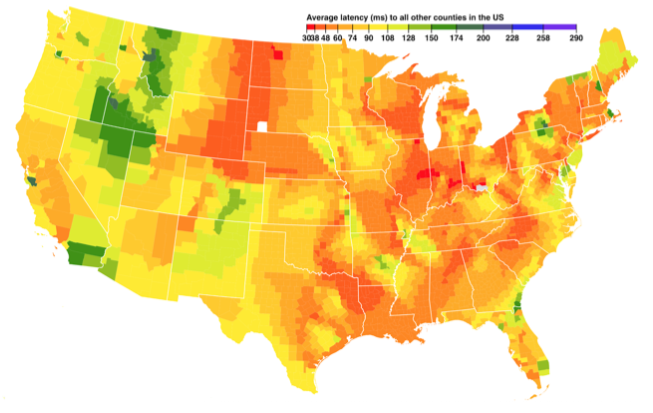
\includegraphics[width=0.75\textwidth]{dns/prior_mqp/dns-map.png}
    \caption{Interpolated DNS map from "The Internet Connected Project"\cite{Fakult2019}}
    \label{fig:interpolated_dns_map}
\end{figure}
% \end{wrapfigure}

The concept of \dns cache manipulation was ultimately used in our own research in evaluating and ranking internet connectivity, discussed in \cref{sec:dns}.

\subsection{Physical Mapping of Fiber-Optic Networks in the United States}
In 2015 researchers at the University of Wisconsin (Madison) mapped locations of fiber backbone within the \us, attempting to understand how the backbone was influenced by existing infrastructure (e.g. railroads and highways). They found strong correlation between the location of fiber lines and the locations of major roads built in the mid 20th century. This result is significant for internet connectivity because it further highlights that cities that were well connected physically during the industrial revolution continue to be the best connected \cite{Durairajan2015a}.
 